\item[(c)]
\section*{Task (c)}

\subsection*{Problem Statement}
Now the so-called short-time Fourier Transform (STFT) should be implemented. To this end, the total signal is grouped into overlapping blocks of a specified length, and each block is transformed individually into the frequency domain. Additionally, the individual blocks should be filtered using a Hamming window (MATLAB command `hamming`) for improving the spectral illustration.

\begin{itemize}
    \item Implement the generation of the signal blocks given the total signal. Every block should have a length of 256 samples. Use an overlapping factor of 2, i.e., every block is overlapping with its preceding block by half the signal length. The last block should also have a length of 256 samples; if not enough samples from the total signal are left to obtain a block of length 256, append the appropriate number of zeros.
    \item Every block should be multiplied with a Hamming window. The window can be generated with the MATLAB command `hamming`.
    \item Transform the windowed blocks to the frequency domain using the FFT to obtain the Fourier transformed blocks (FTBs).
    \item Plot a 2D diagram showing the FTBs. For this purpose, consider which frequency values have to be displayed on the frequency axis, and which time values have to be plotted on the time axis, i.e., which frequency range has been regarded with the FFTs and at which points in time have the FFTs of the individual blocks been computed? Generate two MATLAB vectors \( f_{\text{stft}} \) and \( t_{\text{stft}} \), which contain the appropriate frequency and time values, respectively. Then, plot the diagram containing the magnitude of the STFT result using the MATLAB command `surface(t_{\text{stft}}, f_{\text{stft}}, abs(stft_mtx))`, where `stft_mtx` is the matrix containing the individual FTBs. Display the amplitude information with the command `colorbar`. The STFT magnitude diagram in your protocol should look similar to Fig. 2 (the symbol sequence might not be the same), where in Fig. 2 only the frequency range 0–2000 Hz is shown.
\end{itemize}

\subsection*{Python Script}
\begin{verbatim}
import numpy as np
import matplotlib.pyplot as plt
from scipy.io import wavfile
from scipy.signal import hamming
import os

# Create fig directory if it doesn't exist
if not os.path.exists('fig'):
    os.makedirs('fig')

# Read the DTMF signal from the WAV file
fs, signal = wavfile.read('dtmf.wav')

# Parameters for STFT
block_length = 256  # Block length
overlap = block_length // 2  # Overlapping factor of 2
window = hamming(block_length)  # Hamming window

# Pad the signal with zeros if necessary
padding_length = (block_length - len(signal) % block_length) % block_length
padded_signal = np.append(signal, np.zeros(padding_length))

# Generate signal blocks
num_blocks = (len(padded_signal) - overlap) // (block_length - overlap)
blocks = np.zeros((num_blocks, block_length))

for i in range(num_blocks):
    start = i * (block_length - overlap)
    end = start + block_length
    blocks[i, :] = padded_signal[start:end] * window

# Compute the FFT for each block
ftbs = np.fft.fft(blocks, axis=1)

# Generate the time and frequency vectors for plotting
f_stft = np.fft.fftfreq(block_length, 1/fs)[:block_length // 2]
t_stft = np.arange(num_blocks) * (block_length - overlap) / fs

# Plot the STFT magnitude
plt.figure(figsize=(12, 6))
plt.pcolormesh(t_stft, f_stft, np.abs(ftbs[:, :block_length // 2].T), shading='gouraud')
plt.title('STFT Magnitude of DTMF Signal')
plt.xlabel('Time (s)')
plt.ylabel('Frequency (Hz)')
plt.colorbar(label='Magnitude')
plt.ylim(0, 2000)  # Limit the frequency range to 0-2000 Hz
plt.savefig('fig/ex4_c_stft_magnitude.png')
plt.show()
\end{verbatim}

\subsection*{STFT Magnitude of the DTMF Signal}
\begin{figure}[h]
    \centering
    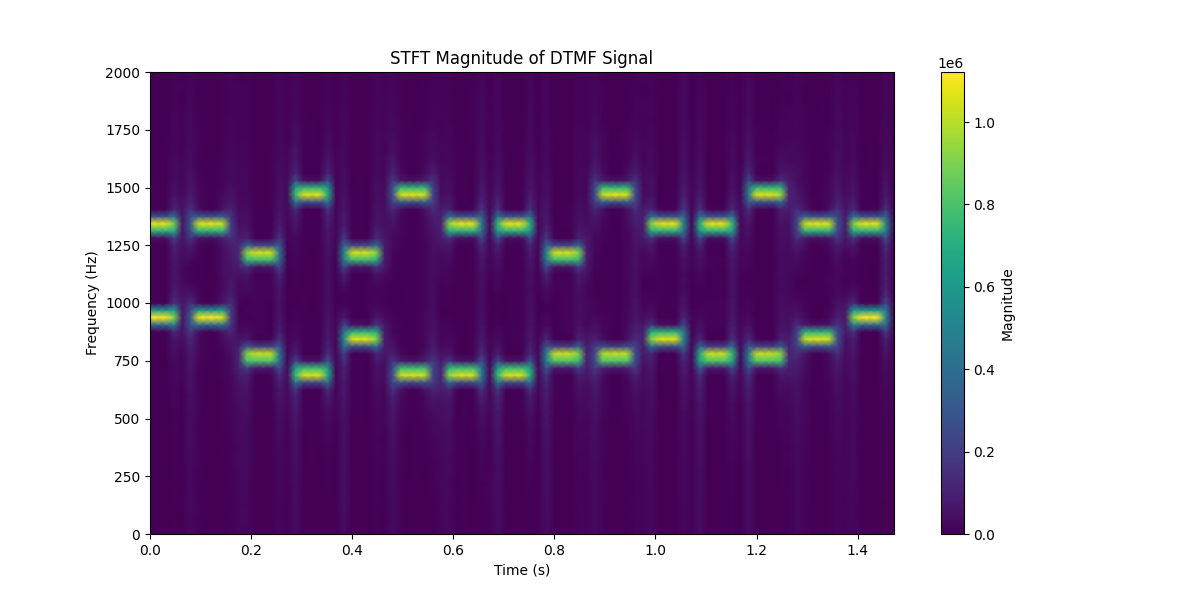
\includegraphics[width=0.8\textwidth]{fig/ex4_c_stft_magnitude.png}
    \caption{STFT Magnitude of the DTMF Signal}
    \label{fig:ex4_c_stft_magnitude}
\end{figure}

\subsection*{Analysis}
The STFT magnitude plot provides a time-frequency representation of the DTMF signal. Each block is transformed individually into the frequency domain, and the overlapping blocks are windowed with a Hamming window to improve the spectral illustration.
